\chapter{Introduction\label{sec:intro}}

%Standard Model
% - What does it consist of (particles, interactions, gauge fields)
% - Description of Higgs mechanism and its significance
% - Examples of SM limitations (DM, gravity, Higgs loop corrections...)

%Supersymmetry
% - What is supersymmetry, what SM problems does it address
% - 2HDM, NMSSM: Motivations
% - 

\subsection{The Standard Model\label{sec:SM}}

Elementary particle physics is the study of the most fundamental components of matter: determining what these components are, and also how they behave. The word ``atom" is derived from the ancient Greek word for ``indivisible"; the discovery that atoms are not in fact indivisible but are themselves made up of smaller components -- electrons, protons, and neutrons -- set the stage for the ongoing search for ever-smaller and more fundamental building blocks of matter. This has culminated in the present day with the Standard Model, a quantum field theory that provides the most successful description to date of all experimentally observed fundamental particles and their interactions. In this framework, fundamental particles are interpreted as excitations of quantum fields, and interactions between particles occur via the exchange of mediating particles~\cite{BettiniPhysics}. This chapter will present an overview of the Standard Model, its deficiencies, and the theory of supersymmetry that has been developed to address some of these deficiencies.

\subsubsection{A little background\label{sec:SM-history}}

Classical physics differentiates clearly between matter particles, which behave as pointlike objects, and radiation, which behaves as a wave. The discovery of phenomena such as the photoelectric effect and the Compton effect, which point to the quantization radiation, challenged classical assumptions about the wave behaviour of radiation. Similarly, observations of diffraction behaviour in electron beams revealed that treating particles as pointlike bodies is not sufficient, and that beams of electrons can in fact behave like waves~\cite{MessiahPhysics}. The quest to understand this wave-particle duality led to the development of quantum mechanics to describe physical phenomena at the microscopic scale.

In quantum mechanics, the physical state of a particle or system of particles is characterized by a wavefunction, which depends on the particle coordinates in space and time. Measurable properties of particles (such as position and momentum) and the evolution of the physical state of the system can all be derived from operations on the wavefunction. The wavelike behaviour of particles at this scale is reflected in the plane-wave wavefunction for free particles, and the bound-state wavefunctions that are related to standing waves, with discrete (quantized) energy levels available to the particles in the bound system.

Quantum field theory goes a step further from dealing with systems of wavelike particles, by treating particles themselves as quantized excitations of fields~\cite{PeskinSchroederPhysics}. The operation of a field operator in a vacuum at a particular position and time represents the production of a particle at that position and time, and interactions between particles occur via couplings to gauge fields, vector fields whose excitations (also referred to as gauge bosons) are the mediators of the fundamental interactions associated with those fields.

The development of the Standard Model has led to predictions of the existence of a variety of new particles, and over the decades, high-energy physics experiments have confirmed the existence of these particles. The following section presents a summary of the current state of the Standard Model and its categorization of all known fundamental particles to date.

\subsubsection{Particles of the Standard Model\label{sec:SM-particles}}

Fundamental particles can be classified into three main categories: leptons, quarks, and gauge bosons. Fig.~\ref{fig:StandardModelTable} illustrates the classification of particles in the Standard Model.

\begin{figure}
   \begin{center}
      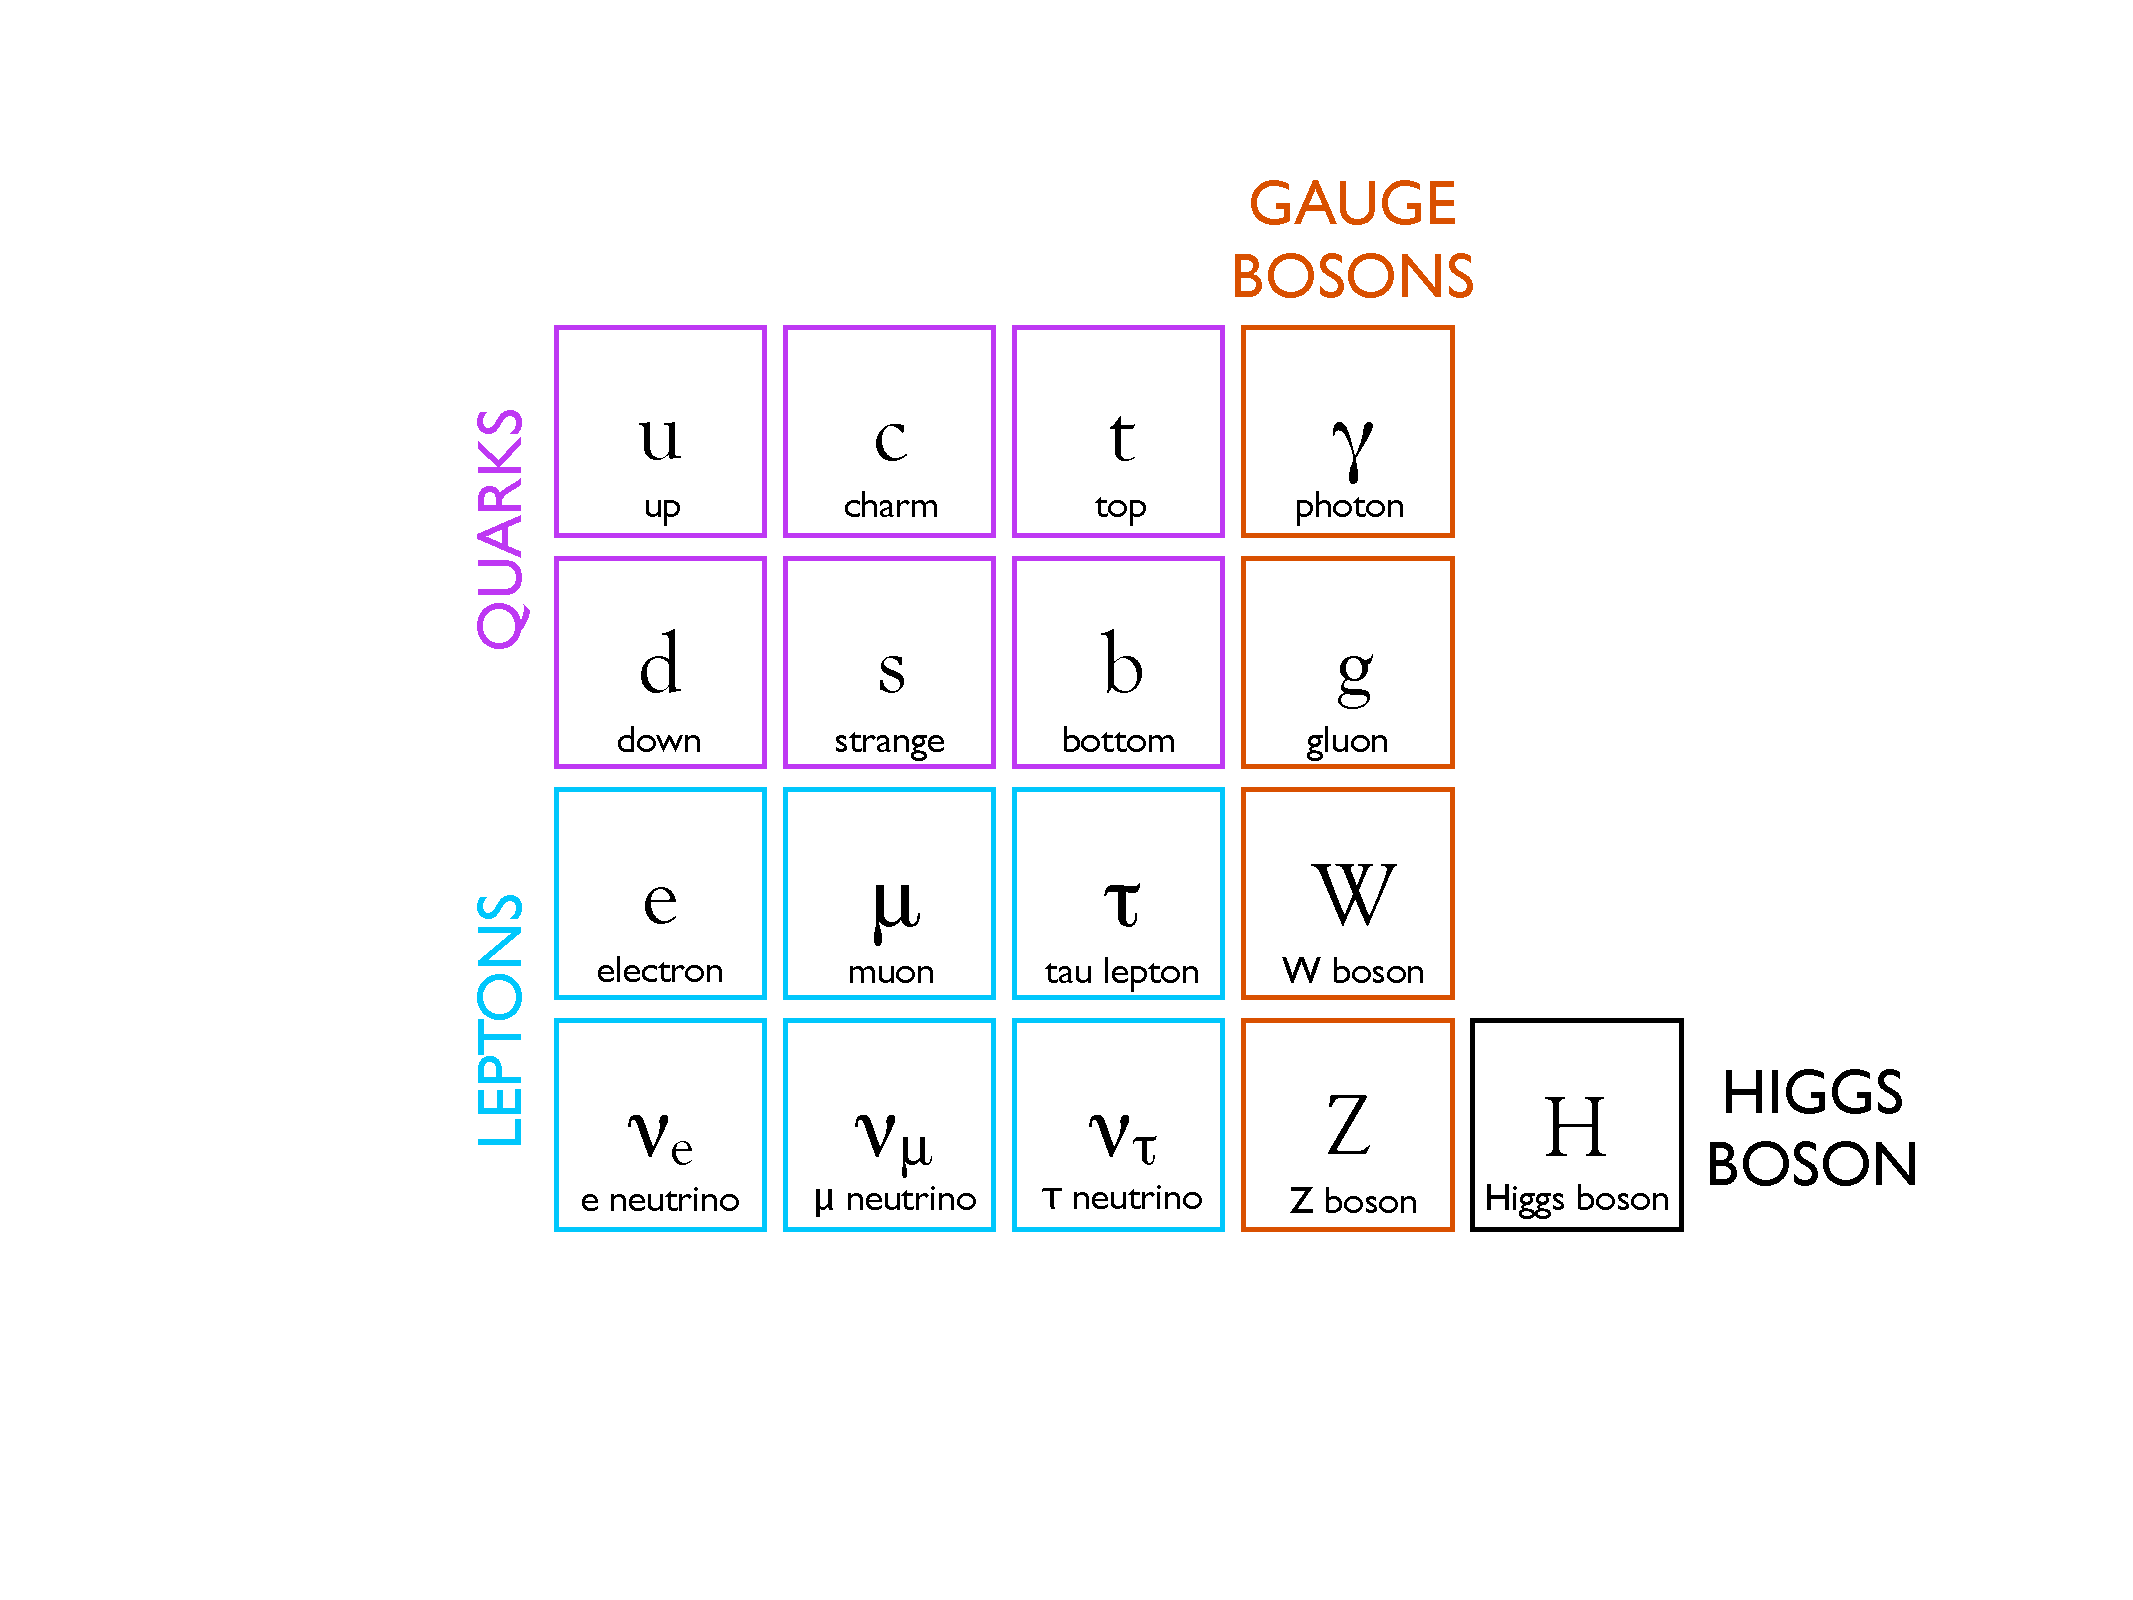
\includegraphics[width=0.6\textwidth]{figures/StandardModelTable}
      \caption{Standard Model particles.}
      \label{fig:StandardModelTable}
   \end{center}
\end{figure}

The leptons and quarks are all fermions -- particles with half-integer spin whose dynamics obey the Dirac equation. Leptons have integer electric charge and fall into three generations called ``flavours". The negatively charged leptons are the electron, the muon, and the tau (in increasing order of mass), and each is associated with a massless neutrino; for each lepton, there is also an associated antiparticle. Quarks have fractional electric charge and fall into three generations; there are a total of six quark flavours (two per generation), and quarks also possess another quantum property known as ``colour", whose implications will be explained shortly.

Particles interact via four fundamental forces: the strong force, electromagnetism, the weak force, and gravity. These interactions are mediated by gauge bosons, which obey Bose-Einstein statistics and have integer spin. Any particle with electric charge can participate in electromagnetic interactions, which are mediated by electrically neutral, massless photons. The strong force is mediated by gluons, which are colorless, electrically neutral, and massless; only quarks and gluons, which possess nonzero colour charge, can participate in strong interactions. W$^{\pm}$ or Z$^{0}$ bosons are the carriers of the weak force, which is responsible for such processes as nuclear decays (they will hence be referred to as $W$ and $Z$, dropping the charge superscript unless it is necessary to explicitly mention their charges). Unlike the gluon and photon, the $W$ and $Z$ bosons are massive.
%flavour: , each of which can be regarded as a representation of the SU(2)$\times$U(1) group
%colour: , which can be regarded as representations of the SU(3) group

The dynamics of quantum mechanical processes such as transitions between states are described by a function called the Lagrangian $\mathcal{L}$. By Noether's theorem, the symmetry of a Lagrangian under the transformations of a symmetry group implies the conservation of some quantity. The conservation of electric charge, for instance, results from the invariance of the electromagnetic Lagrangian under U(1) transformations. Fundamental interactions are governed by the symmetry of their Lagrangians under gauge transformations, with transitions between states constrained by the conservation of quantum numbers associated with the mediating interaction. Gauge bosons come from the generators of the symmetry group, each of which gives rise to a corresponding gauge field.

The Standard Model belongs to the symmetry group SU(3)$\times$SU(2)$\times$U(1). The invariance of the QCD portion of the Lagrangian under the SU(3) gauge group requires that gluons, the generators of the SU(3) symmetry, be massless. The electroweak portion of the Lagrangian belongs to the SU(2)$\times$U(1) gauge group; the gauge fields $B_{\mu}$ (from the U(1) group) and \textbf{W}$^1$$_{\mu}$, \textbf{W}$^2$$_{\mu}$, and \textbf{W}$^3$$_{\mu}$ (from the SU(2) group) give rise to gauge bosons that mediate electroweak interactions~\cite{Bednyakov:2007pz}. The mass terms in the Lagrangian for the electroweak gauge bosons violate local SU(2)$\times$U(1) gauge invariance; therefore, the masses of the electroweak gauge bosons would have to be zero. However, this presents a problem, because although the photon is known to be massless, the W and Z bosons that mediate the weak force have been experimentally proven to be massive.

This paradox is resolved by the concepts of spontaneous symmetry breaking and the Higgs mechanism~\cite{ThomsonPhysics}. This involves the introduction of a complex scalar field whose vacuum expectation value is not zero but instead one of multiple nonzero minima of the scalar field potential. The choice of one of these vacuum expectation values will break the symmetry of the scalar potential. When the Lagrangian of such a scalar field is expressed in terms of a perturbation of the field about its vacuum expectation value, this results in a mass term for the perturbation that corresponds to a scalar boson called a Goldstone boson.

To complete the picture, the spontaneous symmetry of the scalar field is embedded in the SU(2)$\times$U(1) symmetry; this results in what is known as the Higgs mechanism. The simplest model requires two complex scalar fields. When the combined Lagrangian of the scalar fields and electroweak gauge fields is expressed as an expansion about the chosen vacuum expectation values of the scalar fields, one ends up with terms quadratic in the $B_{\mu}$, \textbf{W}$^1$$_{\mu}$, \textbf{W}$^2$$_{\mu}$, and \textbf{W}$^3$$_{\mu}$ fields. Via an appropriate gauge transformation, the Goldstone bosons resulting from the symmetry breaking disappear by being absorbed into the longitudinal degree of freedom of the \textbf{W}$^i$$_{\mu}$ fields, and the mixing of the four gauge fields results in the W$^{\pm}$ bosons, which are linear combinations of \textbf{W}$^1$$_{\mu}$ and \textbf{W}$^2$$_{\mu}$, and a Z boson and a photon, both of which are linear combinations of \textbf{W}$^3$$_{\mu}$ and $B_{\mu}$. When this mixing is accounted for in the Lagrangian, the only mass terms that remain are the ones for the W and Z bosons, while the photon is massless. The existence of the Higgs field also generates the masses of the fermions via Yukawa interactions between fermions and the Higgs field in the electroweak Lagrangian.

\subsection{Deficiencies of the Standard Model\label{sec:SMdeficiencies}}

Although the Standard Model has been successful in describing a wide range of experimental results, it also falls short in many respects. To name a few of them~\cite{BettiniPhysics}:

\begin{itemize}
\item \textbf{Gravity: }The four fundamental forces are the strong force, electromagnetism, the weak force, and gravity. The Standard Model accounts for the first three, but the way in which gravity, which is $10^{-32}$ times weaker than the weak force, factors into the Standard Model is still unknown.
\item \textbf{Neutrino oscillations: }The Standard Model treats neutrinos as massless particles. However, there is strong experimental evidence to the contrary. The observation of neutrino flavour oscillations, which cannot occur if neutrinos were massless, suggests that the observed electron, muon, and tau neutrino flavours are not in fact mass eigenstates -- rather, the observed neutrino flavour states are superpositions of mass eigenstates. What the mass eigenvalues are and why they are so small, are mysteries that remain to be resolved.
\item \textbf{Dark matter and energy: }Matter constitutes only about 30\% of the total mass-energy density of the universe; the remainder is comprised of ``dark matter" and ``dark energy", but their exact nature is unknown, and their presence is only deduced indirectly from their gravitational effects, since dark matter does not emit or absorb electromagnetic radiation. Thus, it is suspected that dark matter must be made up of some different type of particle not accounted for by the Standard Model.
\item \textbf{Grand unification: }The running coupling constants of the strong, electromagnetic, and weak interactions generally approach one another at increasingly higher energy scales. This suggests that these three fundamental interactions (and perhaps also gravity) might be manifestations of one unified field theory and thus may unify at some high energy scale; some theories predict this scale to be on the order of 10$^{16}$ GeV.
\item \textbf{The hierarchy problem: }The Standard Model predicts that the mass of the Higgs boson receives loop corrections from leptons, quarks, and whatever other particles may couple to the Higgs. As a result, the Higgs mass would be expected to receive corrections up to the order of the Planck scale ($\mathcal{O}$(10$^{19}$ GeV)) at which gravity becomes significant and the Standard Model of physics no longer holds. The fact that the magnitude of the actual Higgs mass is so much lower than those of the predicted corrections is surprising, as it implies that there must be some mechanism by which these corrections are cancelled. This constitutes what is known as the hierarchy problem of the Standard Model.
\end{itemize}

These deficiencies indicate that the Standard Model is not a complete theory, and that more elements are needed to provide a more accurate description of nature.

\subsection{Supersymmetry}

One theory that has been proposed to address the hierarchy problem is that there exists a certain symmetry -- called supersymmetry -- that relates fermions to bosons~\cite{Martin:1997ns}. For each fermion, there would exist a corresponding bosonic parter particle, and likewise for each boson there would exist a fermionic partner; such partner particles are referred to as superpartners. Under a supersymmetric transformation, a fermion turns into its superpartner and vice versa. Thus, for each loop correction to the Higgs mass, there would be another loop correction from the supersymmetric partner particle; since fermionic loops have a sign opposite that of bosonic loops, the loop corrections would cancel neatly.

As supersymmetry posits a superpartner for every Standard Model particle, it is of great interest to look for experimental evidence of these superpartners, as none have yet been observed. The masses of supersymmetric particles are not specified, but the numerous parameters of the theory can be constrained by experimental measurements.

The simplest model incorporating supersymmetry into the Standard Model is the Minimal Supersymmetric Standard Model (MSSM)~\cite{Martin:1997ns}. The details will not be covered here, but the Higgs sector consists of two chiral Higgs supermultiplets $H_u$ and $H_d$, of which the former couples to up-type quarks and the latter couples to down-type quarks and charged leptons. The superpotential W$_{MSSM}$ of the MSSM, which defines the most general non-gauge interactions for the superfields, is:

\begin{equation}
W_{MSSM} = \bar{u}y_{u}QH_{u} - \bar{d}y_{d}QH_{d} - \bar{e}y_{e}LH_{d} + \bar{\mu}H_{u}H_{d}
\label{eq:WMSSM}
\end{equation}

While the MSSM does provide a cancellation of large corrections to the Higgs mass, it comes with deficiencies of its own. One problem, called the $\mu$-problem, stems from the fact that the $\mu$ coupling constant in Equation~\ref{eq:WMSSM} should be of the order of magnitude of the electroweak scale in order to provide the Higgs doublets with nonzero vacuum expectation values after electroweak symmetry breaking, but its magnitude is expected to be more naturally close to the Planck scale, which is significantly larger. Fine-tuning its magnitude to that of the electroweak scale thus seems arbitrary and without physical motivation.

The $\mu$-problem is circumvented in the Next-to-Minimal Supersymmetric Standard Model (NMSSM), which adds a scalar Higgs singlet field S to the Higgs sector of the MSSM and thus predicts a total of seven Higgs bosons -- a pair of charged ones, three neutral scalars, and two neutral pseudoscalars. The NMSSM superpotential is:

\begin{equation}
W_{NMSSM} = W_{MSSM} + \lambda SH_{u}H_{d} + \frac{1}{3}\kappa S^3 + \frac{1}{2}\mu_{s}S^2
\label{eq:WNMSSM}
\end{equation}

The coupling of the singlet field $S$ to the doublet fields naturally generates an effective $\mu$ term equal to $\lambda$$<S>$, with the desired magnitude near the electroweak scale. The fact that the NMSSM circumvents the $\mu$-problem makes it of great interest to study. The new physics search presented in this thesis is a probe into the Higgs sector of the NMSSM.